% !TeX program = pdflatex
% !BIB program = biber



\addvspace{2\baselineskip plus 0.67\baselineskip}
% Because for some reason, \parnotes removes the vertical space before the following section heading

\section{Methods}
\label{sec:Methods}

In this section, we first present the design of the experiment (\ref{sec:design}) and derive behavioral predictions (\ref{sec:Predictions}).

\subsection{Design of the Main Experiment}
\label{sec:design}

\subsubsection{General Features}
\blindtext

\subsubsection{More Specific Features}
\blindtext

\begin{figure}[tp!]
	\RawFloats
	\centering
	% !TeX TS-program = pdflatex
% !BIB program = biber



\providecommand{\twolines}{}
\renewcommand{\twolines}[2]{$
	\displaystyle
	\begin{array}{c} \\[-3.1ex]
		#1 \\
		+ \\
		#2
	\end{array}
$}

%\providecommand{\xA}{-11.5}
%\providecommand{\xB}{ -8.5}
%\providecommand{\xC}{ -5.5}
%\providecommand{\xD}{ -2.5}
%\providecommand{\xE}{  0.5}
%\providecommand{\xF}{  3.5}
%\providecommand{\xG}{  6.5}
%\providecommand{\xH}{  9.5}
%\providecommand{\xI}{ 12.5}
%\providecommand{\xJ}{ 15.5}
%\providecommand{\xJ}{ 15.5}
\providecommand{\xA}{-12.0}
\providecommand{\xB}{-10.5}
\providecommand{\xC}{ -8.0}
\providecommand{\xD}{ -5.5}
\providecommand{\xE}{ -3.0}
\providecommand{\xF}{ -0.5}
\providecommand{\xG}{  2.0}
\providecommand{\xH}{  4.5}
\providecommand{\xI}{  7.0}
\providecommand{\xJ}{  9.5}
\providecommand{\xX}{ 12.5}

\providecommand{\yAA}{- 0.75}
\providecommand{\yAB}{- 3.70}
\providecommand{\yDA}{- 4.50}
\providecommand{\yDB}{- 7.45}
\providecommand{\yCA}{- 8.25}
\providecommand{\yCB}{-11.20}
\providecommand{\yBA}{-12.00}
\providecommand{\yBB}{-14.95}


%\afterpage{%
%\begin{landscape}

% \begin{figure}[t]
	% \scalebox{0.5}{
	\resizebox{0.9\textwidth}{!}{%
		\begin{tikzpicture}[scale = 0.7]

		% Crop the tikzpicture to avoid unnecessary whitespace around it:
		\path[use as bounding box, red] (\xA-2.1, 1.5) rectangle (\xJ+0.8, \yBB-0.4);

		\draw[->] (\xB - 0.75, 0) -- (\xJ + 0.75,0);
		\node at  (\xJ + 0.7, 0.4) {$t$};

		\node[below] at (0.5*\xB+0.5*\xC, 1.4) {$w$ weeks};
		\path[->] (\xB,0.275) edge [bend left] (\xC, 0.275);

		\node[below] at (0.5*\xE+0.5*\xF, 1.4) {$w$ weeks};
		\path[->] (\xE,0.275) edge [bend left] (\xF, 0.275);

		\draw (\xB,0.075) -- (\xB,-0.075); %node at (\xB,0.3) {$1$};
		\draw (\xC,0.075) -- (\xC,-0.075); %node at (\xC,0.3) {$2$};
		\draw (\xD,0.075) -- (\xD,-0.075); %node at (\xD,0.3) {$3$};
		\draw (\xE,0.075) -- (\xE,-0.075); %node at (\xE,0.3) {$4$};
		\draw (\xF,0.075) -- (\xF,-0.075); %node at (\xF,0.3) {$5$};
		\draw (\xG,0.075) -- (\xG,-0.075); %node at (\xG,0.3) {$6$};
		\draw (\xH,0.075) -- (\xH,-0.075); %node at (\xH,0.3) {$7$};
		\draw (\xI,0.075) -- (\xI,-0.075); %node at (\xI,0.3) {$8$};
		\draw (\xJ,0.075) -- (\xJ,-0.075); %node at (\xJ,0.3) {$9$};

		% Gray horizontal separation lines:
		\draw[gray] (\xB-0.75, \yBA+0.4) -- (\xJ+0.75, \yBA+0.4);
		\draw[gray] (\xB-0.75, \yCA+0.4) -- (\xJ+0.75, \yCA+0.4);
		\draw[gray] (\xB-0.75, \yDA+0.4) -- (\xJ+0.75, \yDA+0.4);
		\draw[gray] (\xB-0.75, \yBB-0.3) -- (\xJ+0.75, \yBB-0.3);

		\node[below, text width = 3cm] at (\xA, \yAA+0.125) {$\CbalA$:};

		\node[below] at (\xB, \yAA) {\twolines{1}{B\,(1 - x)}}; % {$1$}
		\node[above] at (\xB, \yAB) {\huge{\textcolor{darkblue}{$\downarrow$}}};
		\node[below] at (\xC, \yAA) {$1$};
		\node[below] at (\xD, \yAA) {$1$};
		\node[below] at (\xE, \yAA) {$1$};
		\node[below] at (\xF, \yAA) {$1$};
		\node[below] at (\xG, \yAA) {$1$};
		\node[below] at (\xH, \yAA) {$1$};
		\node[below] at (\xI, \yAA) {$1$};
		\node[below] at (\xJ, \yAA) {\twolines{1}{R\,B\,x}};
		\node[above] at (\xJ, \yAB) {\huge{\textcolor{darkblue}{$\uparrow$}}};

		\node[below, text width = 3cm] at (\xA, \yBA+0.125) {$\CunbalA[8]$:};

		\node[below] at (\xB, \yBA) {\twolines{1}{B\,(1 - x)}};
		\node[above] at (\xB, \yBB) {\huge{\textcolor{darkblue}{$\downarrow$}}};
		\node[below] at (\xC, \yBA) {\twolines{1}{R\,B\,x\mathop{/}8}};
		\node[above] at (\xC, \yBB) {\large{\textcolor{darkblue}{$\uparrow$}}};
		\node[below] at (\xD, \yBA) {\twolines{1}{R\,B\,x\mathop{/}8}};
		\node[above] at (\xD, \yBB) {\large{\textcolor{darkblue}{$\uparrow$}}};
		\node[below] at (\xE, \yBA) {\twolines{1}{R\,B\,x\mathop{/}8}};
		\node[above] at (\xE, \yBB) {\large{\textcolor{darkblue}{$\uparrow$}}};
		\node[below] at (\xF, \yBA) {\twolines{1}{R\,B\,x\mathop{/}8}};
		\node[above] at (\xF, \yBB) {\large{\textcolor{darkblue}{$\uparrow$}}};
		\node[below] at (\xG, \yBA) {\twolines{1}{R\,B\,x\mathop{/}8}};
		\node[above] at (\xG, \yBB) {\large{\textcolor{darkblue}{$\uparrow$}}};
		\node[below] at (\xH, \yBA) {\twolines{1}{R\,B\,x\mathop{/}8}};
		\node[above] at (\xH, \yBB) {\large{\textcolor{darkblue}{$\uparrow$}}};
		\node[below] at (\xI, \yBA) {\twolines{1}{R\,B\,x\mathop{/}8}};
		\node[above] at (\xI, \yBB) {\large{\textcolor{darkblue}{$\uparrow$}}};
		\node[below] at (\xJ, \yBA) {\twolines{1}{R\,B\,x\mathop{/}8}};
		\node[above] at (\xJ, \yBB) {\large{\textcolor{darkblue}{$\uparrow$}}};%

		\node[below, text width = 3cm] at (\xA, \yCA+0.125) {$\CunbalA[4]$:};

		\node[below] at (\xB, \yCA) {\twolines{1}{B\,(1 - x)}};
		\node[above] at (\xB, \yCB) {\huge{\textcolor{darkblue}{$\downarrow$}}};
		\node[below] at (\xC, \yCA) {$1$};
		\node[below] at (\xD, \yCA) {$1$};
		\node[below] at (\xE, \yCA) {$1$};
		\node[below] at (\xF, \yCA) {$1$};
		\node[below] at (\xG, \yCA) {\twolines{1}{R\,B\,x\mathop{/}4}};
		\node[above] at (\xG, \yCB) {\Large{\textcolor{darkblue}{$\uparrow$}}};
		\node[below] at (\xH, \yCA) {\twolines{1}{R\,B\,x\mathop{/}4}};
		\node[above] at (\xH, \yCB) {\Large{\textcolor{darkblue}{$\uparrow$}}};
		\node[below] at (\xI, \yCA) {\twolines{1}{R\,B\,x\mathop{/}4}};
		\node[above] at (\xI, \yCB) {\Large{\textcolor{darkblue}{$\uparrow$}}};
		\node[below] at (\xJ, \yCA) {\twolines{1}{R\,B\,x\mathop{/}4}};
		\node[above] at (\xJ, \yCB) {\Large{\textcolor{darkblue}{$\uparrow$}}};%

		\node[below, text width = 3cm] at (\xA, \yDA+0.125) {$\CunbalA[2]$:};

		\node[below] at (\xB, \yDA) {\twolines{1}{B\,(1 - x)}};
		\node[above] at (\xB, \yDB) {\huge{\textcolor{darkblue}{$\downarrow$}}};
		\node[below] at (\xC, \yDA) {$1$};
		\node[below] at (\xD, \yDA) {$1$};
		\node[below] at (\xE, \yDA) {$1$};
		\node[below] at (\xF, \yDA) {$1$};
		\node[below] at (\xG, \yDA) {$1$};
		\node[below] at (\xH, \yDA) {$1$};
		\node[below] at (\xI, \yDA) {\twolines{1}{R\,B\,x\mathop{/}2}};
		\node[above] at (\xI, \yDB) {\LARGE{\textcolor{darkblue}{$\uparrow$}}};
		\node[below] at (\xJ, \yDA) {\twolines{1}{R\,B\,x\mathop{/}2}};
		\node[above] at (\xJ, \yDB) {\LARGE{\textcolor{darkblue}{$\uparrow$}}};
		\end{tikzpicture}%
	}
	\caption{Budget Sets $\CbalA$ and $\CunbalA$}
	% \captionof{figure}{Budget Sets: \balA and \unbalA Conditions}
	\label{fig:incrdisp_bs}
		% with $b\in\{8,11\}$, $r\in\{0.2,0.5,0.8 \}$, $w\in\{2,3,6\}$, $n\in\{2,4,8\}$: \textcolor{red}{12 choices} \\
%	\tablenotes[Note:]{%
%		For the values of $B$, $R$, and $w$ that we used see \autoref{sec:Procedure}.
%		The arrows indicate whether and in which direction payments at the respective payment dates change if the savings rate $x$ is increased.
%	}
% \end{figure}

%\end{landscape}%
%}

	\smallskip
	% !TeX program = pdflatex
% !BIB program = biber


\renewcommand{\twolines}[2]{$
	\displaystyle
	\begin{array}{c} \\[-12.75pt]
	#1 \\
	+ \\
	\displaystyle #2
	\end{array}
	$}

\renewcommand{\xA}{-12.00}
\renewcommand{\xB}{-10.50}
\renewcommand{\xC}{ -8.30}
\renewcommand{\xD}{ -6.10}
\renewcommand{\xE}{ -3.90}
\renewcommand{\xF}{ -1.70}
\renewcommand{\xG}{  0.50}
\renewcommand{\xH}{  2.70}
\renewcommand{\xI}{  4.90}
\renewcommand{\xJ}{  7.10}
\renewcommand{\xX}{  8.00}


\renewcommand{\yAA}{- 0.75}
\renewcommand{\yAB}{- 4.00}
\renewcommand{\yDA}{- 4.75}
\renewcommand{\yDB}{- 8.00}
\renewcommand{\yCA}{- 8.75}
\renewcommand{\yCB}{-12.00}
\renewcommand{\yBA}{-12.75}
\renewcommand{\yBB}{-16.00}

%\afterpage{%
%\begin{landscape}

% \begin{figure}[b]
	% \scalebox{0.5}{
	\resizebox{0.9\textwidth}{!}{
	\begin{tikzpicture}[scale = 0.75]

		\path[use as bounding box, red] (\xA-1.85, 2) rectangle (\xX+0.8,\yBB-0.4);	% To crop the tikzpicture to avoid unnecessary whitespace around it

		\draw[-]      (\xB-0.75,0) -- (\xI+0.75,0);
		\draw[dashed] (\xI+1,0) -- (\xX-1,0);
		\draw[->]     (\xX-0.75,0) -- (\xX+0.75,0);
		\node at      (\xX+0.7, 0.4) {$t$};

		\node[below] at (0.5*\xB+0.5*\xC, 1.4) {$w$ weeks};
		\path[->] (\xB, 0.275) edge [bend left] (\xC, 0.275);

		\node[below] at (0.5*\xE+0.5*\xF, 1.4) {$w$ weeks};
		\path[->] (\xE, 0.275) edge [bend left] (\xF, 0.275);

		\node at (0.5*\xI+0.5*\xX, 1.45) {7~months};
		\path[->] (\xI, 0.275) edge [bend left=45] (\xX, 0.275);


		\draw (\xB,0.075) -- (\xB,-0.075); %node at (\xB,0.3) {$1$};
		\draw (\xC,0.075) -- (\xC,-0.075); %node at (\xC,0.3) {$2$};
		\draw (\xD,0.075) -- (\xD,-0.075); %node at (\xD,0.3) {$3$};
		\draw (\xE,0.075) -- (\xE,-0.075); %node at (\xE,0.3) {$4$};
		\draw (\xF,0.075) -- (\xF,-0.075); %node at (\xF,0.3) {$5$};
		\draw (\xG,0.075) -- (\xG,-0.075); %node at (\xG,0.3) {$6$};
		\draw (\xH,0.075) -- (\xH,-0.075); %node at (\xH,0.3) {$7$};
		\draw (\xI,0.075) -- (\xI,-0.075); %node at (\xI,0.3) {$8$};
		\draw (\xX,0.075) -- (\xX,-0.075); %node at (\xX,0.3) {$9$};

		% Gray horizontal separation lines:
		\draw[gray] (\xB-0.75, \yBA+0.4) -- (\xX+0.75, \yBA+0.4);
		\draw[gray] (\xB-0.75, \yCA+0.4) -- (\xX+0.75, \yCA+0.4);
		\draw[gray] (\xB-0.75, \yDA+0.4) -- (\xX+0.75, \yDA+0.4);
		\draw[gray] (\xB-0.75, \yBB-0.3) -- (\xX+0.75, \yBB-0.3);

	\node[below, text width = 3cm] at (\xA, \yAA+0.115) {$\CbalB$:};

		\node[below] at (\xB, \yAA) {$1$};
		\node[below] at (\xC, \yAA) {$1$};
		\node[below] at (\xD, \yAA) {$1$};
		\node[below] at (\xE, \yAA) {$1$};
		\node[below] at (\xF, \yAA) {$1$};
		\node[below] at (\xG, \yAA) {$1$};
		\node[below] at (\xH, \yAA) {$1$};
		\node[below] at (\xI, \yAA) {\twolines{1}{B\,(1 - x)}};
		\node[above] at (\xI, \yAB) {\huge{\textcolor{darkblue}{$\downarrow$}}};
		\node[below] at (\xX, \yAA) {\twolines{1}{R\,B\,x}};
		\node[above] at (\xX, \yAB) {\huge{\textcolor{darkblue}{$\uparrow$}}};

	\node[below, text width = 3cm] at (\xA, \yDA+0.115) {$\CunbalB[2]$:};

		\node[below] at (\xB, \yDA) {$1$};
		\node[below] at (\xC, \yDA) {$1$};
		\node[below] at (\xD, \yDA) {$1$};
		\node[below] at (\xE, \yDA) {$1$};
		\node[below] at (\xF, \yDA) {$1$};
		\node[below] at (\xG, \yDA) {$1$};
		\node[below] at (\xH, \yDA) {\twolines{1}{\frac{B\,(1 - x)}{2}}};
		\node[above] at (\xH, \yDB) {\LARGE{\textcolor{darkblue}{$\downarrow$}}};
		\node[below] at (\xI, \yDA) {\twolines{1}{\frac{B\,(1 - x)}{2}}};
		\node[above] at (\xI, \yDB) {\LARGE{\textcolor{darkblue}{$\downarrow$}}};
		\node[below] at (\xX, \yDA) {\twolines{1}{R\,B\,x}};
		\node[above] at (\xX, \yDB) {\huge{\textcolor{darkblue}{$\uparrow$}}};

	\node[below, text width = 3cm] at (\xA, \yCA+0.115) {$\CunbalB[4]$:};

		\node[below] at (\xB, \yCA) {$1$};
		\node[below] at (\xC, \yCA) {$1$};
		\node[below] at (\xD, \yCA) {$1$};
		\node[below] at (\xE, \yCA) {$1$};
		\node[below] at (\xF, \yCA) {\twolines{1}{\frac{B\,(1 - x)}{4}}};
		\node[above] at (\xF, \yCB) {\Large{\textcolor{darkblue}{$\downarrow$}}};
		\node[below] at (\xG, \yCA) {\twolines{1}{\frac{B\,(1 - x)}{4}}};
		\node[above] at (\xG, \yCB) {\Large{\textcolor{darkblue}{$\downarrow$}}};
		\node[below] at (\xH, \yCA) {\twolines{1}{\frac{B\,(1 - x)}{4}}};
		\node[above] at (\xH, \yCB) {\Large{\textcolor{darkblue}{$\downarrow$}}};
		\node[below] at (\xI, \yCA) {\twolines{1}{\frac{B\,(1 - x)}{4}}};
		\node[above] at (\xI, \yCB) {\Large{\textcolor{darkblue}{$\downarrow$}}};
		\node[below] at (\xX, \yCA) {\twolines{1}{R\,B\,x}};
		\node[above] at (\xX, \yCB) {\huge{\textcolor{darkblue}{$\uparrow$}}};

	\node[below, text width = 3cm] at (\xA, \yBA+0.115) {$\CunbalB[8]$:};

		\node[below] at (\xB, \yBA) {\twolines{1}{\frac{B\,(1 - x)}{8}}};
		\node[above] at (\xB, \yBB) {\large{\textcolor{darkblue}{$\downarrow$}}};
		\node[below] at (\xC, \yBA) {\twolines{1}{\frac{B\,(1 - x)}{8}}};
		\node[above] at (\xC, \yBB) {\large{\textcolor{darkblue}{$\downarrow$}}};
		\node[below] at (\xD, \yBA) {\twolines{1}{\frac{B\,(1 - x)}{8}}};
		\node[above] at (\xD, \yBB) {\large{\textcolor{darkblue}{$\downarrow$}}};
		\node[below] at (\xE, \yBA) {\twolines{1}{\frac{B\,(1 - x)}{8}}};
		\node[above] at (\xE, \yBB) {\large{\textcolor{darkblue}{$\downarrow$}}};
		\node[below] at (\xF, \yBA) {\twolines{1}{\frac{B\,(1 - x)}{8}}};
		\node[above] at (\xF, \yBB) {\large{\textcolor{darkblue}{$\downarrow$}}};
		\node[below] at (\xG, \yBA) {\twolines{1}{\frac{B\,(1 - x)}{8}}};
		\node[above] at (\xG, \yBB) {\large{\textcolor{darkblue}{$\downarrow$}}};
		\node[below] at (\xH, \yBA) {\twolines{1}{\frac{B\,(1 - x)}{8}}};
		\node[above] at (\xH, \yBB) {\large{\textcolor{darkblue}{$\downarrow$}}};
		\node[below] at (\xI, \yBA) {\twolines{1}{\frac{B\,(1 - x)}{8}}};
		\node[above] at (\xI, \yBB) {\large{\textcolor{darkblue}{$\downarrow$}}};
		\node[below] at (\xX, \yBA) {\twolines{1}{R\,B\,x}};
		\node[above] at (\xX, \yBB) {\huge{\textcolor{darkblue}{$\uparrow$}}};

	\end{tikzpicture}%
	}
	\caption{Budget Sets $\CbalB$ and $\CunbalB$}
	% \captionof{figure}{Budget Sets: \balB and \unbalB Conditions }
	\label{fig:decrdisp_bs}


% \end{figure}

%\end{landscape}%
%}

	\bigskip
	\begin{minipage}{\textwidth}%
		\footnotesize\setlength{\baselineskip}{11pt}%
		\textit{Notes:} For the values of $B$, $R$, and $w$ that we used, see \autoref{sec:Procedure}. The savings rate~$x$ is individuals' choice variable: they choose some $x \in \mathbfit{X} = {\{0, \sfrac{1}{100}, \sfrac{2}{100}, \dots, 1\}}$ in each trial.
		The arrows indicate whether and in which direction payments at the respective payment dates change if $x$ is increased.
		$\sigma_\epsilon, c^\alpha$.
		This figure was taken from \cite{Dertwinkel-Kalt2017}.
	\end{minipage}
\end{figure}

Let's test the euro symbol: \texteuro, \euro 1,234.56, $\euro 1{,}234.56$. Let's also test text superscripts: $i$\textsuperscript{th} and text subscripts: CO\textsubscript{2} and H\textsubscript{2}O.
$\sigma_\epsilon, c^\alpha$.
\blindtext
Let's test the footnote settings.\footnote{\blindmathfalse\blindtext\blindmathtrue}

\begin{figure}[t]
	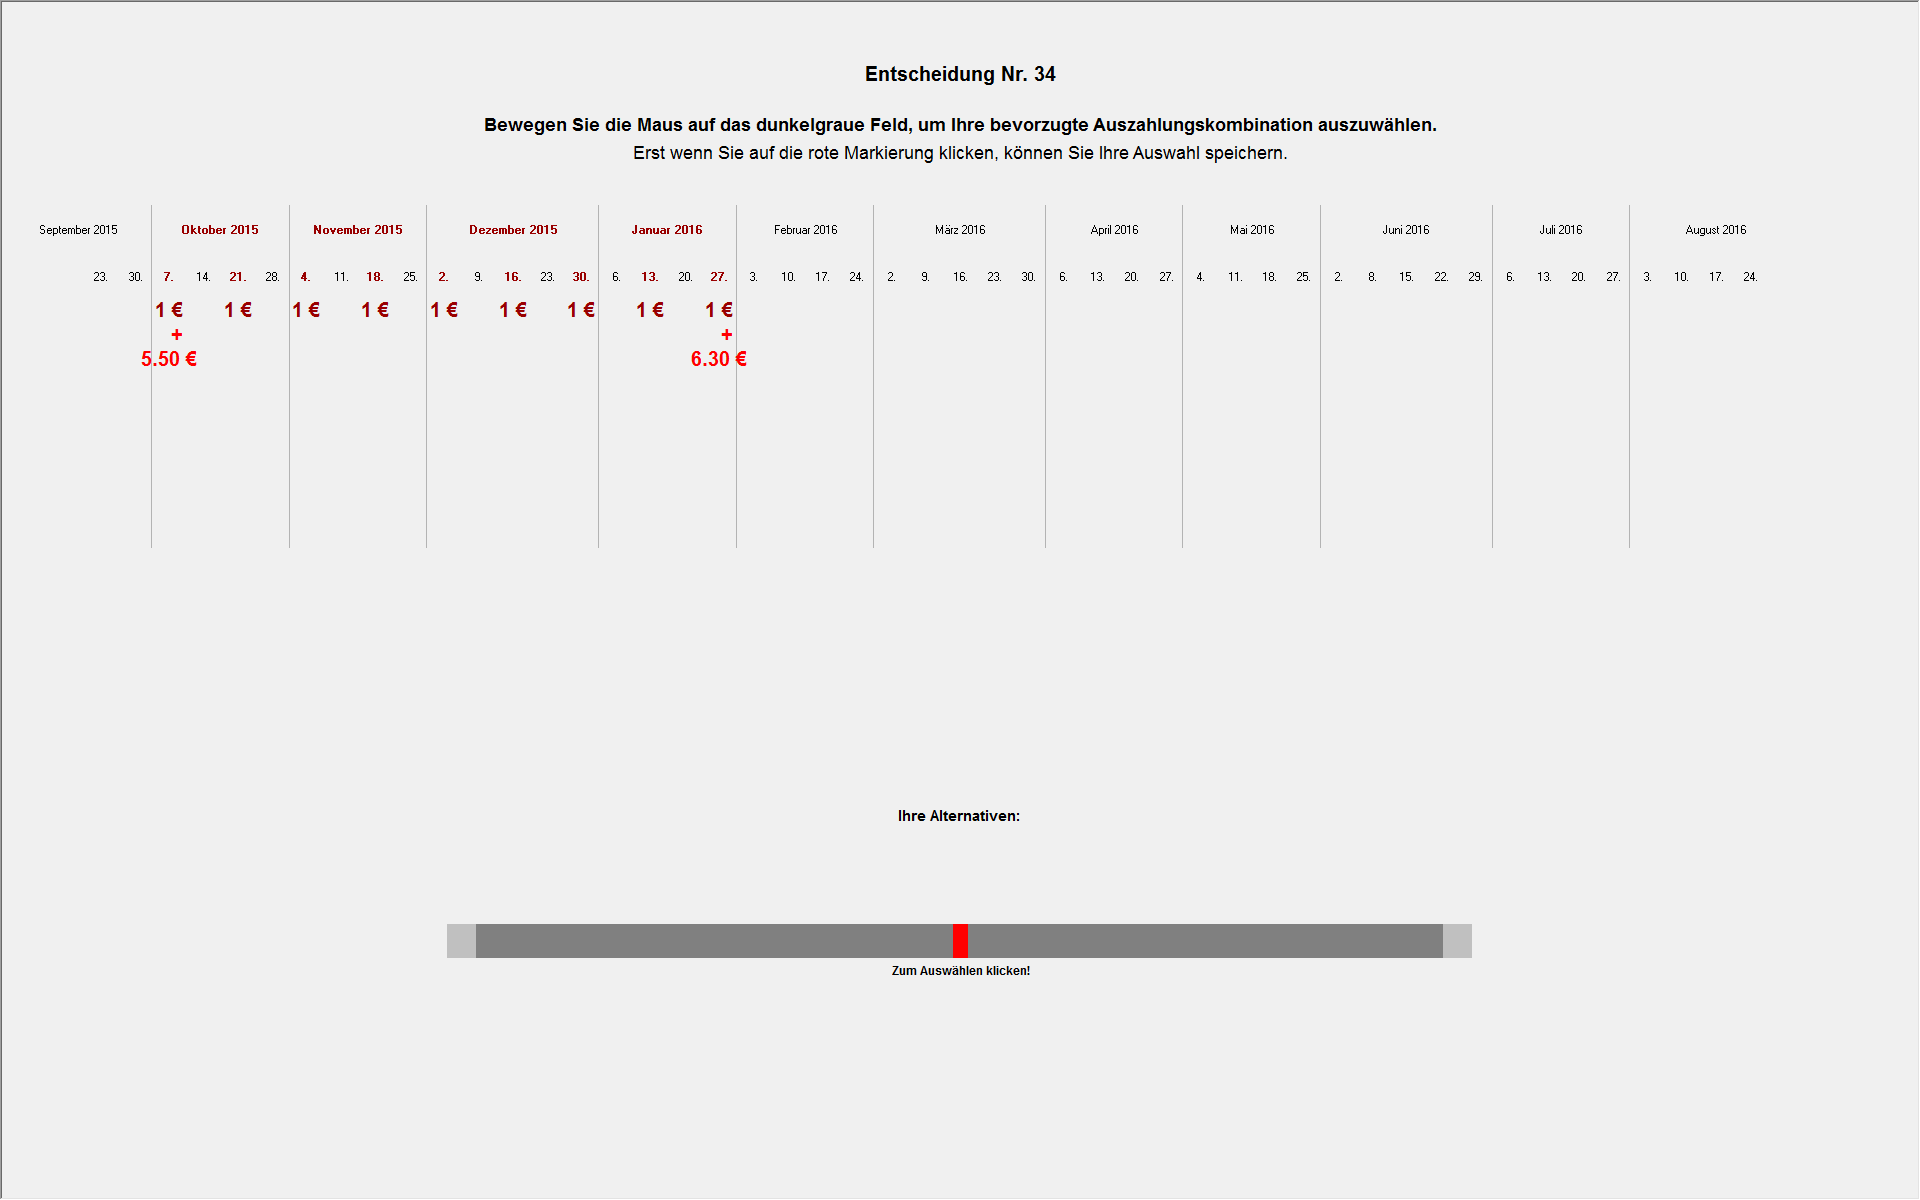
\includegraphics[width=\textwidth]{../Images/Screenshots/BS_inc_conc_half.png} \\[\medskipamount]
	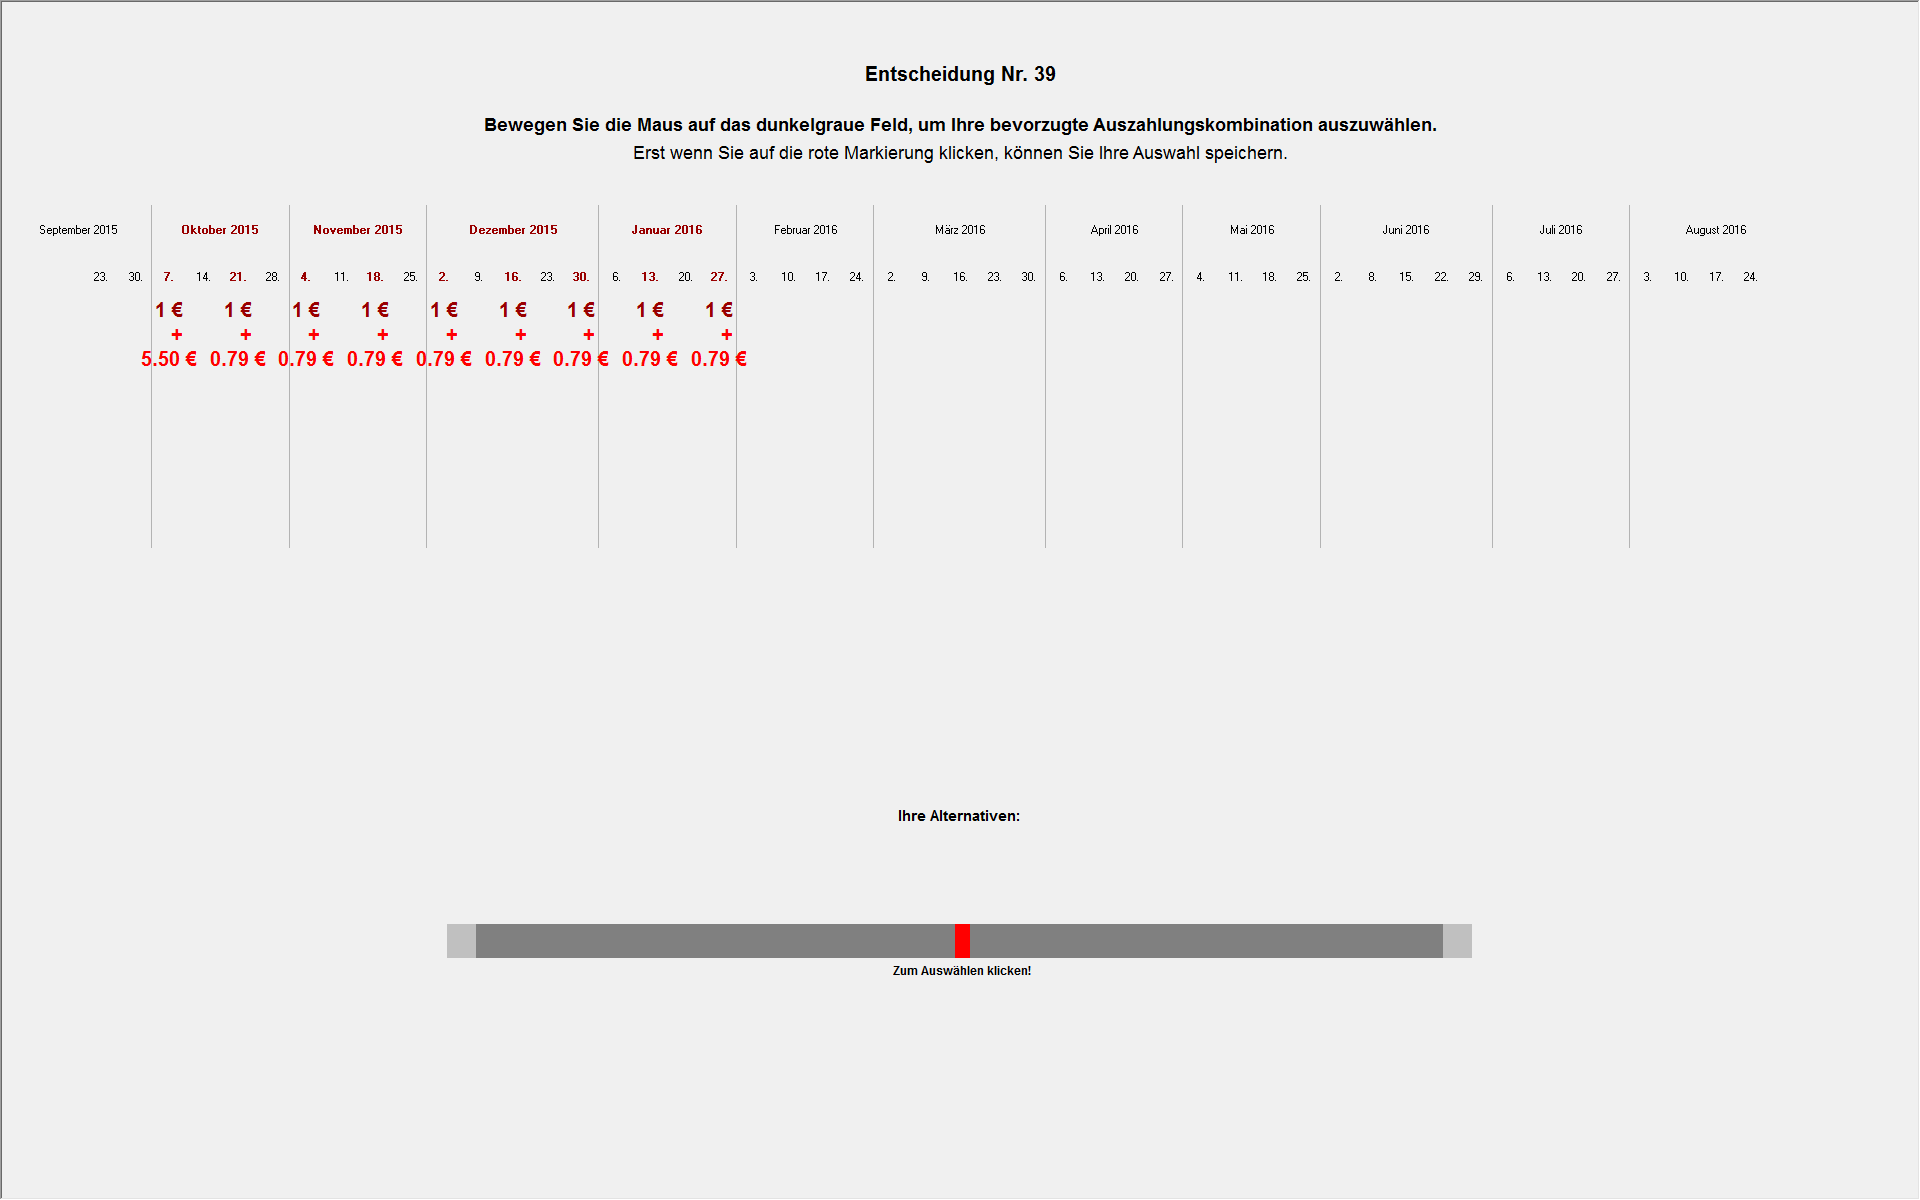
\includegraphics[width=\textwidth]{../Images/Screenshots/BS_inc_disp_half.png}
	\caption{Screenshots of a~\balA Decision (Top) and an~\unbalA[8] Decision (Bottom)%
	}
	\label{fig:screenshot:BS_inc_half}
	\figurenotes[Note:]{%
		This figure was taken from \cite{Dertwinkel-Kalt2017}.
	}
\end{figure}%

\autoref{fig:screenshot:BS_inc_half} shows an~exemplary decision screen with $B=\euro 11$ and $r\approx15\%$ for both \balA (upper panel) and \unbalA[8] (lower panel). Through a~slider, subjects choose their preferred ${x \in \CS[X]}$.\footnote{The slider had no initial position---it appeared only after subjects first positioned the mouse cursor over the slider bar. This was done to avoid default effects.} The slider position in Figure \ref{fig:screenshot:BS_inc_half} indicates ${x = 0.5}$, i.e., the earliest payment is reduced by \euro 5.50. Since ${r \approx 15\%}$ in this example, this slider position amounts to \euro 6.30 that are paid at later payment dates. While these \euro 6.30 are paid in a~single bank transfer on the latest payment date in \balA, the amount is dispersed in equal parts over the last 8~payment dates in \unbalA[8]---i.e., 8~consecutive payments of \euro 0.79.\footnote{We always rounded the second decimal place up so that the sum of the payments included in a~dispersed payoff was always at least as great as the respective concentrated payoff.}

\subsubsection{Some More Details}
\blindtext

Here's a~bulleted list:
\Blindlist{itemize}[3]

\subsubsection{Procedure}
\label{sec:Procedure}
Describe the sequence of events in your study. You could do this with the help of an~enumerated list:
\Blindlist{enumerate}[3]
